\documentclass[11pt,a4paper]{article}
\usepackage[margin=2.4cm]{geometry}
\usepackage[T1]{fontenc}
\usepackage{lmodern}
\usepackage{amsmath,amssymb}
\usepackage{booktabs}
\usepackage{multirow}
\usepackage{graphicx}
\usepackage{siunitx}
\usepackage{microtype}
\usepackage[hidelinks]{hyperref}
\sisetup{group-separator={,},group-minimum-digits=4}
\newcommand{\cfg}[1]{\texttt{#1}}

\title{Whole-frame debris detection in forward-looking sonar\\with integer-only inference on embedded hardware}
\author{Technical report, \texttt{sonar\_edge}}
\date{3 November 2026}

\begin{document}
\maketitle

\begin{abstract}
\noindent
We report a single-stage detector for marine debris in forward-looking sonar
frames, together with its post-training 8-bit quantisation and a
standard-library-only C implementation that reproduces the quantised network
bit for bit. Because the public dataset consists of a few long recordings with
shuffled frame indices, random splits overestimate accuracy; we reconstruct the
recordings from the box annotations and evaluate by five-fold cross-validation
over these scenes with pooled average precision. The deployed configuration
(35~M multiply--accumulates per frame) attains a pooled mAP@0.5 of 49.4\%
(49.7\% after quantisation); a 13$\times$ larger reference attains 55.2\%. Two
ablations separate the factors by which the reference differs: additional
channel width at the same resolution yields no measurable gain ($+0.8$),
whereas the unchanged network at 1.5$\times$ the input resolution recovers
$+5.2$ of the $5.8$ points at 2.25$\times$ the cost. The C runtime processes a
frame of the deployed configuration in 10~ms on one laptop core.
\end{abstract}

\section{Introduction}

Forward-looking sonar (FLS) is the principal sensor for underwater debris
surveys in turbid water, and the detector must typically run on a small
embedded computer on the vehicle. Prior work on the dataset used here
\cite{valdenegro2025} classifies cropped patches; the predecessor study
(\texttt{sonar\_cnn}) reimplemented that pipeline and found that its reported
accuracy depends on near-duplicate frames being shared between training and
test sets. The present work addresses the deployment problem end to end:
whole-frame detection, an evaluation protocol that controls the duplicate
leak, integer-only inference, and a verified C runtime. This report describes
the evaluation protocol (Section~\ref{sec:split}), the detector
(Section~\ref{sec:model}), the integer implementation
(Section~\ref{sec:runtime}) and the results obtained to date
(Section~\ref{sec:results}). The per-milestone documents \texttt{docs/M0}--\texttt{M4}
in the repository contain the complete derivations and intermediate results.

\section{Data}
\label{sec:data}

The water-tank subset of the marine debris FLS dataset \cite{valdenegro2025}
comprises 1\,868 frames recorded with an ARIS Explorer 3000 and projected to
Cartesian coordinates at $320 \times 480$ pixels (width $\times$ height), single
channel, 8 bit. Each frame carries between one and five Pascal-VOC bounding
boxes (3\,882 in total) in eleven classes. Ten classes are debris objects; the
eleventh, \emph{Wall}, marks the tank walls. It is retained as a detector
class, since a deployed system must not report walls as debris, but excluded
from the scene reconstruction of Section~\ref{sec:split}, because walls are
static and would link unrelated recordings.

The frames originate from a small number of recordings during which the sonar
drifts slowly over a fixed arrangement of objects, so that consecutive frames
are near-duplicates. The published frame indices carry no temporal
information: the median thumbnail correlation of index-adjacent pairs (0.757)
equals that of random pairs (0.747), and 2\% of adjacent pairs have fully
matching box layouts, as do random pairs. A split by frame therefore places
near-identical frames on both sides of the split, and the resulting test score
measures memorisation of the recording rather than generalisation to new
arrangements.

\section{Evaluation protocol}
\label{sec:split}

\subsection{Scene reconstruction}

Since the recording order cannot be recovered from metadata, it is
reconstructed from the annotations. For two frames $A$ and $B$ with Wall boxes
removed, the \emph{layout match} from $A$ to $B$ is defined as
\begin{equation}
  m(A \to B) = \frac{1}{|A|}\,\bigl|\{\, p \in A : \exists\, q \in B,\;
  \mathrm{cls}(q) = \mathrm{cls}(p),\; \mathrm{IoU}(p, q) \ge 0.5 \,\}\bigr| ,
\end{equation}
the fraction of boxes in $A$ that have a same-class box in $B$ at
intersection-over-union of at least $0.5$ in original pixel coordinates. Two
frames are \emph{linked} if and only if
\begin{equation}
  m(A \to B) = 1 \quad\text{and}\quad m(B \to A) = 1 ,
\end{equation}
that is, every object in either frame has a counterpart in the other. Frames
without non-wall boxes are linked to nothing. \emph{Scenes} are the connected
components of the link graph over all $\binom{1868}{2}$ pairs, computed by
union--find. Linkage is transitive by construction: the first and last frames
of a long recording need not match directly, but are joined through the
intermediate frames.

Both the full-match requirement and the exclusion of walls are necessary.
Requiring every box to match in both directions prevents chaining through a
single shared object. With Wall boxes included, or with the required fraction
relaxed from $1$ to $0.5$, 1\,686 of the 1\,868 frames collapse into one
component. The procedure yields 191 scenes, the largest containing 201, 158,
158, 119 and 90 frames; 118 scenes consist of a single frame, mostly frames
whose only boxes are walls. Random members of four scenes of different sizes
were inspected visually; each is one physical arrangement of objects observed
under small changes of viewpoint and gain.

\subsection{Illustration}

Figure~\ref{fig:pairs} shows frame 18 and three other frames;
Table~\ref{tab:pairs} gives the corresponding matching terms. Frames 18 and
187 are linked directly: each of the three objects matches at IoU between
0.71 and 0.85. Frame 151 belongs to the same scene (scene 176, fold 4) but is
not linked to frame 18 directly, the sonar having drifted until no box pair
reaches IoU 0.5; the two frames are joined through intermediate frames. Frame
124 contains the same two bottles at nearly the same positions but no tire, so
that $m(18 \to 124) = 2/3$ and the pair is not linked; it belongs to scene 10,
which lies in fold 3.

\begin{figure}[t]
  \centering
  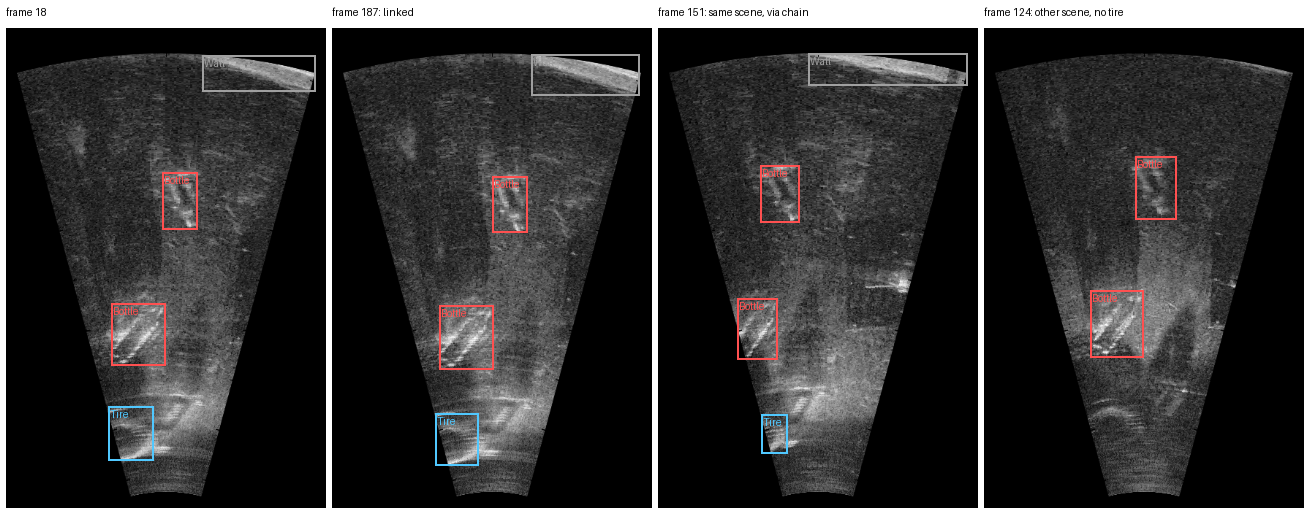
\includegraphics[width=\textwidth]{fig/pairs.png}
  \caption{Frame 18 and three partner frames with their annotations (red:
  bottle, blue: tire, grey: wall). Frames 18 and 187 are linked directly;
  frame 151 belongs to the same scene through intermediate frames; frame 124
  belongs to a different scene because the tire is absent.}
  \label{fig:pairs}
\end{figure}

\begin{table}[t]
  \centering
  \small
  \begin{tabular}{llcccl}
    \toprule
    Pair & Box in frame 18 $(x,y,w,h)$ & Best same-class IoU & $m(18\to B)$ & $m(B\to 18)$ & Outcome \\
    \midrule
    18, 187 & Bottle (156,144,35,57) & 0.71 & \multirow{3}{*}{$3/3$} & \multirow{3}{*}{$3/3$} & \multirow{3}{*}{linked} \\
            & Bottle (105,275,54,62) & 0.85 & & & \\
            & Tire   (102,378,45,54) & 0.76 & & & \\
    \midrule
    18, 151 & Bottle (156,144,35,57) & 0.00 & \multirow{3}{*}{$0/3$} & \multirow{3}{*}{$0/3$} & not linked directly; \\
            & Bottle (105,275,54,62) & 0.16 & & & same scene (176, fold 4) \\
            & Tire   (102,378,45,54) & 0.42 & & & through intermediate frames \\
    \midrule
    18, 124 & Bottle (156,144,35,57) & 0.56 & \multirow{3}{*}{$2/3$} & \multirow{3}{*}{$2/2$} & not linked; \\
            & Bottle (105,275,54,62) & 0.71 & & & scene 10, fold 3 \\
            & Tire   (102,378,45,54) & --   & & & \\
    \bottomrule
  \end{tabular}
  \caption{Layout-matching terms for the pairs of Figure~\ref{fig:pairs}. A
  pair is linked only when both fractions equal 1.}
  \label{tab:pairs}
\end{table}

The third pair exhibits the known limitation of the procedure. Frame 124 is
plausibly the same physical setup recorded before the tire was placed. The
rule cannot establish this, assigns the frame to a separate scene, and that
scene falls into a different fold, so that background texture is shared across
the fold boundary. The error is in the conservative direction: too few links
make the evaluation stricter, never more lenient, which is why the procedure
is accepted as it stands.

\subsection{Fold assignment}

The 191 scenes are assigned to $K = 5$ folds by a deterministic greedy
procedure. Scenes are processed in order of decreasing size, and each is
assigned to the fold that minimises, after the assignment, the sum over
classes of the squared share of that class's boxes plus the squared share of
all frames. The assignment is stored in \texttt{splits/scene\_folds\_v1.json}
and fixed for all experiments. Table~\ref{tab:folds} gives the resulting fold
sizes and class shares. Balance is limited by the data: several classes occur
almost entirely within one scene (94\% of standing-bottle boxes, 66\% of
valve, 54\% of drink-carton), and a scene is never divided. Fold 3 is the
smallest because it carries the standing-bottle scene.

\begin{table}[h]
  \centering
  \small
  \begin{tabular}{lccccc}
    \toprule
    & Fold 0 & Fold 1 & Fold 2 & Fold 3 & Fold 4 \\
    \midrule
    Scenes & 34 & 39 & 38 & 43 & 37 \\
    Frames & 439 & 388 & 383 & 230 & 428 \\
    \midrule
    Bottle & 43\% & 12\% & 6\% & 3\% & 36\% \\
    Can & 22\% & 18\% & 24\% & 3\% & 33\% \\
    Chain & 14\% & 15\% & 22\% & 37\% & 11\% \\
    Drink-carton & 24\% & 54\% & 6\% & 2\% & 14\% \\
    Hook & 23\% & 30\% & 13\% & 6\% & 28\% \\
    Propeller & 32\% & 23\% & 22\% & 5\% & 18\% \\
    Shampoo-bottle & 7\% & 10\% & 35\% & 5\% & 42\% \\
    Standing-bottle & 3\% & 0\% & 3\% & 94\% & 0\% \\
    Tire & 34\% & 39\% & 9\% & 3\% & 15\% \\
    Valve & 2\% & 17\% & 66\% & 5\% & 10\% \\
    Wall & 17\% & 25\% & 16\% & 18\% & 24\% \\
    \bottomrule
  \end{tabular}
  \caption{Fold composition: number of scenes and frames, and the share of
  each class's boxes, per fold.}
  \label{tab:folds}
\end{table}

\subsection{Development split and cross-validation}

Model development uses a single split: fold 0 as test set, fold 1 as
validation set for epoch selection, and folds 2--4 as training set
(1\,041 / 388 / 439 frames).

Final results are obtained by five-fold cross-validation. For $k = 0, \dots,
4$, a model is trained from random initialisation with fold $k$ as test set,
fold $(k+1) \bmod 5$ as validation set and the remaining three folds as
training set; for $k = 2$, for instance, folds 4, 0 and 1 are used for
training, fold 3 for selection and fold 2 for testing. Every scene is thus
tested exactly once, by a model that has seen none of its frames. The five
test prediction sets partition the dataset and are scored jointly as a single
detection problem (\emph{pooled} average precision, following the VOC
convention). Pooling is the only estimate defined for classes concentrated in
one scene: standing-bottle is testable only in the run that holds out fold 3,
whose training set contains four instances of the class, and pooling reports
the resulting precision without averaging over four undefined per-fold
values. The mean and standard deviation of the per-fold mAP are reported
alongside as a measure of fold-to-fold variation. Both the floating-point
model and its 8-bit quantisation are evaluated under this protocol, since the
C runtime reproduces the latter exactly (Section~\ref{sec:runtime}).

GPU training is not bit-reproducible. A seed-identical repeat of the deployed
configuration on the development split changed the test mAP by 3.8 points;
single-split differences of this magnitude are therefore not interpreted, and
configurations are compared only under cross-validation.

\section{Detector}
\label{sec:model}

\subsection{Architecture}

The detector is a single-stage, anchor-free network in the CenterNet style
\cite{zhou2019}, restricted to operations that a minimal integer runtime can
execute: a sequence of $3 \times 3$ convolutions, each followed by batch
normalisation and ReLU, without residual connections or upsampling, and a
$1 \times 1$ output convolution. The output stride is 8, so that a $480 \times
320$ input produces a $60 \times 40$ grid and a $240 \times 160$ input a $30
\times 20$ grid. Dilation in the later layers enlarges the receptive field to
about 255 input pixels without further downsampling. Table~\ref{tab:configs}
lists the configurations used in this report.

\begin{table}[h]
  \centering
  \small
  \setlength{\tabcolsep}{4pt}
  \begin{tabular}{llcccrrr}
    \toprule
    Configuration & Layers (channels; s2 = stride 2, d$k$ = dilation $k$) & Input & Grid & Params & MACs & RF \\
    \midrule
    \cfg{small} & 16s2, 32s2, 32s2, 32, 32d2, 32d4 & $240{\times}160$ & $30{\times}20$ & \num{42463} & \SI{34.8}{M} & 254 \\
    \cfg{small}, scale 4/3 & as above & $360{\times}240$ & $45{\times}30$ & \num{42463} & \SI{78.4}{M} & 254 \\
    \cfg{small\_wide} & 16s2, 32s2, 64s2, 64, 64d2, 64d4 & $240{\times}160$ & $30{\times}20$ & \num{135359} & \SI{90.4}{M} & 254 \\
    \cfg{base} & 16s2, 32s2, 48s2, 48, 48d2, 48d4, 48d8 & $480{\times}320$ & $60{\times}40$ & \num{102831} & \SI{283.7}{M} & 255 \\
    \cfg{wide} & 16s2, 32s2, 64s2, 64, 64d2, 64d4, 64d8 & $480{\times}320$ & $60{\times}40$ & \num{172351} & \SI{450.2}{M} & 255 \\
    \bottomrule
  \end{tabular}
  \caption{Network configurations. Each layer is a $3{\times}3$ convolution
  with batch normalisation and ReLU (stride 1 and dilation 1 unless marked);
  the head is a $1{\times}1$ convolution to $C + 4 = 15$ channels. RF denotes
  the receptive field in pixels of the full-resolution frame; MACs are
  multiply--accumulates per frame. \cfg{small} is the deployed configuration.}
  \label{tab:configs}
\end{table}

For each grid cell the head outputs $C = 11$ class logits, the box size
$(w, h)$ in units of the stride, and the centre offset $(\delta_x, \delta_y)
\in [0, 1)$ within the cell. The class-logit bias is initialised to $-2.19$
(initial probability $\approx 0.01$) as in \cite{zhou2019}. The input is the
8-bit frame scaled to $[0, 1]$; the half-resolution configurations average
$2 \times 2$ pixel blocks, and the $4/3$ scale applies a box-filter resize.

\subsection{Targets and loss}

For each ground-truth box with centre $(c_x, c_y)$ and size $(w, h)$ in grid
units, a Gaussian is rendered into the target heatmap of its class, centred on
the cell $(\lfloor c_x \rfloor, \lfloor c_y \rfloor)$, with the radius of
\cite{law2018}, the largest displacement at which the displaced box retains
IoU $\ge 0.7$ with the original; overlapping Gaussians are merged by maximum.
Size and offset targets are defined at the centre cell only. The training
objective is
\begin{equation}
  \mathcal{L} = \mathcal{L}_\text{heat} + 0.1\,\mathcal{L}_\text{size} + \mathcal{L}_\text{off},
\end{equation}
where $\mathcal{L}_\text{heat}$ is the penalty-reduced pixelwise focal loss of
\cite{zhou2019} ($\alpha = 2$, $\beta = 4$, normalised by the number of
objects) applied to the sigmoid of the logits, and the regression terms are
L1 losses at the object cells, likewise normalised.

\subsection{Inference}

Detections are the local maxima of the logit heatmap: a cell is retained if
its value is greater than or equal to those of its $3 \times 3$ neighbours
(a max-pooling comparison; no non-maximum suppression is applied). The $K =
32$ highest peaks over all classes are selected, peaks below the logit
threshold $-4$ (probability $\approx 0.018$) discarded, and each remaining peak
at cell $(i_x, i_y)$ converted to a box by
\begin{equation}
  c_x = (i_x + \delta_x)\,s, \qquad c_y = (i_y + \delta_y)\,s, \qquad
  \bigl[c_x - \tfrac{w s}{2},\; c_y - \tfrac{h s}{2},\; c_x + \tfrac{w s}{2},\; c_y + \tfrac{h s}{2}\bigr],
\end{equation}
with $s$ the stride. The decoder operates on logits rather than probabilities;
the sigmoid being monotone, this allows the integer runtime to apply the
threshold to its raw head output.

\subsection{Training}

Networks are trained with AdamW (weight decay $10^{-4}$) under a one-cycle
learning-rate schedule with peak $2 \times 10^{-3}$ and 10\% warm-up, batch
size 16, seed 0, for 150 epochs. The epoch with the highest validation mAP is
selected and the test fold evaluated once. Augmentation comprises horizontal
flipping, integer translation of up to 8 pixels, random scaling by a factor in
$[0.75, 1.3]$ about a random point with probability 0.7 (boxes scaled,
clipped, and discarded when less than 30\% of their area or 4 pixels remain),
additive Gaussian noise with standard deviation drawn from $U[0, 0.04]$,
multiplicative gain in $[0.7, 1.3]$ and additive bias in $[-0.1, 0.1]$. On the
development split, the scaling and noise terms account for an improvement of
about 5 mAP points; lengthening the schedule without them had no effect.

The metric is average precision at IoU 0.5 with all-point interpolation,
computed per class and averaged over the classes present in the evaluated set.
The implementation (\texttt{metrics.py}) is used unchanged to score the C
runtime.

\section{Integer inference}
\label{sec:runtime}

\subsection{Quantisation}

Batch normalisation is folded into the preceding convolution,
$W' = W\gamma/\sqrt{\sigma^2 + \epsilon}$ and $b' = \beta -
\mu\gamma/\sqrt{\sigma^2+\epsilon}$ per output channel, so that the runtime
contains no normalisation layer. The affine scheme of \cite{jacob2018} is used
in its symmetric, zero-point-free form. Every activation is either an input
pixel or a ReLU output, hence non-negative, and is represented as an unsigned
8-bit integer with zero point 0 and one scale $s_a$ per layer. Weights are
signed 8-bit with one scale per output channel, $s_{w,c} = \max|W'_c| / 127$.
With input scale $s_\text{in}$ and output scale $s_\text{out}$, a layer
computes, per output channel $c$,
\begin{equation}
  \mathrm{acc} = \sum_i W_{q,c,i}\, a_{q,i} + b_{q,c}, \qquad
  b_{q,c} = \operatorname{round}\!\Bigl(\frac{b'_c}{s_{w,c}\, s_\text{in}}\Bigr), \qquad
  \mathrm{out}_q = \operatorname{clip}\!\Bigl(\operatorname{round}\bigl(\mathrm{acc}\cdot \tfrac{s_{w,c}\, s_\text{in}}{s_\text{out}}\bigr),\, 0,\, 255\Bigr),
\end{equation}
where the clip implements the ReLU. The real multiplier is replaced by an
integer $M_c \in [2^{30}, 2^{31})$ and a shift $n_c$ with $M_c 2^{-n_c}$
approximating it to a relative error below $10^{-8}$; requantisation is thus
a 64-bit multiplication, the addition of $2^{n_c-1}$ (rounding half away from
zero) and a shift. The $1 \times 1$ head is not requantised: its 32-bit
accumulators are returned with their per-channel real scale and decoded
directly. Activation scales are calibrated as the 99.99th percentile of the
post-ReLU outputs over 64 training frames, divided by 255.

A reference implementation evaluates the integer network with
double-precision tensor operations. This is exact: every product is below
$2^{15}$ and every sum has fewer than $2^{12}$ terms, so all intermediates are
integers well below $2^{53}$. The reference therefore constitutes a bit-exact
specification of the runtime that is fast enough to evaluate a complete test
fold, and it exports the weight tables and three golden input--output pairs.

\subsection{C runtime}

The runtime is written in C11 using only the standard library and is built
with GNU make under \texttt{-std=c11 -O2 -Wall -Wextra -Werror -pedantic}. It
comprises about 165 lines of code and a generated header containing the
8-bit kernels, 32-bit biases, the $(M_c, n_c)$ pairs, the layer table and the
tensor geometry as preprocessor constants. All memory is static: two
activation buffers that alternate as input and output, and the 32-bit head
map. The weights of \cfg{small} occupy 42~KB.

Activations are stored in HWC order (channels innermost) with a zero border
equal to the dilation $d$ of the consuming layer, so that a $3 \times 3$
convolution with stride $s$ reads, for output $(o_y, o_x)$ and tap $(k_y,
k_x)$, the padded pixel $(o_y s + k_y d,\; o_x s + k_x d)$ without bounds
checks, reproducing \texttt{padding = dilation} in PyTorch. Each tap is a dot
product over $c_\text{in}$ contiguous activation bytes and $c_\text{in}$
contiguous weights. Accumulation is in 32-bit integers ($|\mathrm{acc}| <
2^{28}$), requantisation in 64-bit; only non-negative quantities are shifted,
so the implementation-defined right shift of negative integers in C is never
invoked.

The decoder scans each class's 32-bit logit map for cells that are greater
than or equal to their existing $3 \times 3$ neighbours (equivalent to
\texttt{max\_pool2d} with its implicit $-\infty$ padding), converts the score
to a real value in the same operation order as the Python reference, and
forms the box in double precision with the same expression order as the
Python decoder. These per-detection scalar operations are the only
floating-point arithmetic in the runtime. The interface is
\begin{verbatim}
int se_detect(const uint8_t *frame, float thr, se_detection_t *out, int max_out);
const int32_t *se_forward(const uint8_t *frame);   /* int32 head map, HWC */
\end{verbatim}
and a command-line tool reads 8-bit PGM frames and prints one detection per
line.

\subsection{Verification}

Two tests establish the equivalence of the C runtime with the Python
reference. The golden test compares the complete 32-bit head map produced by
\texttt{se\_forward} on the three exported frames with the reference and
requires equality on every one of the $30 \times 20 \times 15$ values. The
end-to-end test runs the compiled binary over the full development test fold
and scores its output with the same metric and ground truth as the Python
models; the C runtime obtains 65.17\% mAP against 65.16\% for the Python
reference, the residual arising from the ordering of detections with exactly
equal scores. The accuracy of the deployed system is consequently established
by the cross-validation of Section~\ref{sec:results}, and only its speed and
energy consumption remain to be measured on the target device.

On a single core of a laptop processor (AMD Ryzen 5 5600H, scalar code,
\texttt{-O2}), the deployed configuration processes one frame in \SI{10}{ms},
corresponding to about 3.5~GMAC/s. The Raspberry Pi 4 is expected to require
35--50~ms per frame; this measurement awaits hardware.

\section{Results}
\label{sec:results}

\subsection{Development split}

Table~\ref{tab:dev} reports the development-split results of the
configurations trained with the protocol of Section~\ref{sec:model}. These
single-run values guided the choice of configuration and are subject to the
run-to-run variation quantified in Section~\ref{sec:split}; the final row is a
seed-identical repeat of the deployed configuration.

\begin{table}[h]
  \centering
  \small
  \begin{tabular}{lcrccc}
    \toprule
    Configuration & Input & MACs & Val.\ mAP & Test mAP, float & Test mAP, int8 / C \\
    \midrule
    \cfg{base} & $480{\times}320$ & 284 M & 66.1 & 63.1 & -- \\
    \cfg{small} (deployed) & $240{\times}160$ & 35 M & 55.0 & 64.1 & 65.2 / 65.17 \\
    \cfg{wide} & $480{\times}320$ & 450 M & 67.8 & 68.8 & -- \\
    \cfg{small}, repeat & $240{\times}160$ & 35 M & 59.9 & 60.3 & -- \\
    \bottomrule
  \end{tabular}
  \caption{Development-split results (mAP@0.5 in \%; fold 0 test, fold 1
  validation; 150 epochs).}
  \label{tab:dev}
\end{table}

\subsection{Cross-validation}

Table~\ref{tab:cv} reports the pooled cross-validation results and the
per-fold test mAP of each configuration; Table~\ref{tab:cvclass} gives the
pooled per-class average precision.

\begin{table}[h]
  \centering
  \small
  \begin{tabular}{lrcccl}
    \toprule
    Configuration & MACs & Pooled, float & Pooled, int8 & Fold mean (s.d.) & Per-fold float, folds 0--4 \\
    \midrule
    \cfg{small} (deployed) & 35 M & 49.4 & 49.7 & 56.4 (8.9) & 60.3, 59.3, 49.9, 44.9, 67.4 \\
    \cfg{small}, $360{\times}240$ & 78 M & 54.6 & 53.7 & 59.5 (9.3) & 64.0, 66.5, 52.3, 47.0, 67.7 \\
    \cfg{small\_wide} & 90 M & 50.2 & 49.6 & 58.0 (11.9) & 60.1, 63.3, 51.1, 42.2, 73.4 \\
    \cfg{wide} & 450 M & 55.2 & 56.2 & 62.8 (8.3) & 66.9, 68.6, 55.7, 52.1, 70.5 \\
    \bottomrule
  \end{tabular}
  \caption{Five-fold cross-validation (mAP@0.5 in \%, pooled over all 1\,868
  frames).}
  \label{tab:cv}
\end{table}

\begin{table}[h]
  \centering
  \small
  \setlength{\tabcolsep}{4pt}
  \begin{tabular}{lrrrrrr}
    \toprule
    Class (boxes) & \cfg{small} & \cfg{small}, int8 & \cfg{small} $360{\times}240$ & \cfg{small\_wide} & \cfg{wide} & \cfg{wide}, int8 \\
    \midrule
    Bottle (468) & 78.0 & 77.4 & 84.2 & 55.9 & 84.7 & 82.7 \\
    Can (292) & 9.1 & 9.6 & 16.1 & 8.3 & 18.8 & 20.5 \\
    Chain (320) & 32.5 & 32.3 & 41.4 & 38.3 & 29.8 & 30.2 \\
    Drink-carton (347) & 62.4 & 64.1 & 69.8 & 69.2 & 81.4 & 79.8 \\
    Hook (171) & 90.8 & 91.4 & 93.6 & 95.0 & 95.5 & 94.9 \\
    Propeller (197) & 51.2 & 50.9 & 49.1 & 47.6 & 46.7 & 46.9 \\
    Shampoo-bottle (111) & 27.7 & 25.5 & 37.6 & 42.0 & 30.5 & 31.4 \\
    Standing-bottle (65) & 1.2 & 2.5 & 3.7 & 2.0 & 24.1 & 26.7 \\
    Tire (615) & 86.8 & 86.8 & 84.4 & 84.0 & 93.9 & 92.7 \\
    Valve (240) & 22.8 & 23.2 & 38.6 & 28.8 & 17.5 & 27.5 \\
    Wall (1056) & 81.3 & 83.4 & 82.6 & 81.0 & 84.8 & 84.9 \\
    \midrule
    mAP, pooled & 49.4 & 49.7 & 54.6 & 50.2 & 55.2 & 56.2 \\
    \bottomrule
  \end{tabular}
  \caption{Pooled per-class average precision (\%) under five-fold
  cross-validation; floating-point models unless marked int8.}
  \label{tab:cvclass}
\end{table}

\section{Discussion}

\paragraph{Protocol.} Pooled cross-validation values lie 10--15 points below
the development-split values of the same configurations. The fold ranking is
identical for every configuration (folds 0, 1 and 4 are easier, folds 2 and 3
harder), which indicates that the per-fold spread is a property of the data
rather than of the models, and that the development fold is among the easier
ones. The per-fold standard deviation of 8--12 points is therefore not a
measure of model uncertainty; the seed-identical repeat on a single split (3.8
points) is the relevant noise figure for comparing configurations.

\paragraph{Resolution versus width.} \cfg{wide} exceeds \cfg{small} by 5.8
pooled points and does so on every fold, by 3.1 to 9.3 points, which is
outside the run-to-run variation. Its gain is concentrated in the small and
low-contrast classes (drink-carton $+19$, standing-bottle $+23$, can $+10$,
bottle $+7$, tire $+7$), whose extent at the half-resolution input is close to
the 8-pixel output stride. \cfg{wide} differs from \cfg{small} in input
resolution and in channel width; \cfg{small\_wide} isolates the second factor
and yields a pooled difference of $+0.8$ (float) and $-0.1$ (int8) relative to
\cfg{small}, with per-fold differences between $-2.7$ and $+6.0$, all within
the run-to-run variation. The complementary experiment, the unchanged
\cfg{small} network at $360 \times 240$ (78~M MACs), gains $+5.2$ pooled points
and exceeds \cfg{small} on every fold (by 0.3 to 7.2 points) while trailing
\cfg{wide} on every fold by 2 to 5 points. The improvement of \cfg{wide} is
therefore attributable to input resolution, and 90\% of it is obtained at a
sixth of its cost, within the budget of about 100~M MACs set for the target
device. The gains occur in the same classes (bottle, can, drink-carton) and
additionally in chain, shampoo-bottle and valve; standing-bottle, the class
with the smallest median extent, improves only at full resolution.

\paragraph{Quantisation.} Post-training 8-bit quantisation is neutral for
\cfg{small} and \cfg{wide} (pooled differences of $+0.3$ and $+1.0$). For
\cfg{small\_wide} and for \cfg{small} at $360 \times 240$ it costs between
0.2 and 3.6 points on every fold ($-0.6$ and $-0.9$ pooled), in both cases
concentrated in the shampoo-bottle class. The cause has not been isolated;
the activation ranges and per-channel weight scales do not differ materially
from those of \cfg{small}, and the quantised $360 \times 240$ model remains
4.0 pooled points above the deployed one.

\paragraph{Pooled per-class values.} Pooled AP is sensitive to the score
calibration of the individual fold models, since detections from all five
models are ranked on one list. The bottle AP of \cfg{small\_wide} (55.9 against
78.0 for \cfg{small}) is an instance: its per-fold bottle AP is 36, 78, 54, 84
and 84, and the single poorly calibrated fold-0 model depresses the pooled
value by more than its share of the boxes. The per-fold values are reported
alongside the pooled ones for this reason.

\section{Limitations and further work}

Each cross-validation fold is a single training run; seed repeats under the
full protocol have not been performed. The standing-bottle class is evaluable
only under the one fold assignment that holds out its scene, with four
training instances, and its AP should be read as a property of the dataset.
The Wall class is scored like the others although its boxes are large and
loosely defined. The scene reconstruction errs toward too few links, as the
example of Figure~\ref{fig:pairs} shows; the residual leak of shared
background across folds is believed to be small but has not been quantified.
The deployed configuration remains \cfg{small} at $240 \times 160$; the
$360 \times 240$ variant is the recommended replacement if the latency measured
on the target device permits it, and requires only regenerating the weight
header, since the runtime takes its geometry from that header. Milestones
M0--M4 (protocol, detector, quantisation, runtime, end-to-end verification)
are complete; the measurement of latency and energy on the
Raspberry Pi (M5), for which the runtime cross-compiles with \texttt{make
CC=aarch64-linux-gnu-gcc}, awaits hardware.

\begin{thebibliography}{9}\raggedright
\bibitem{valdenegro2025} M.~Valdenegro-Toro, D.~C.~Padmanabhan, D.~Singh, B.~Wehbe and Y.~Petillot,
  \emph{Marine debris forward-looking sonar datasets}, 2025. Repository
  \texttt{mvaldenegro/marine-debris-fls-datasets}, commit \texttt{4a77998}.
\bibitem{zhou2019} X.~Zhou, D.~Wang and P.~Kr\"ahenb\"uhl, ``Objects as points,'' arXiv:1904.07850, 2019.
\bibitem{law2018} H.~Law and J.~Deng, ``CornerNet: Detecting objects as paired keypoints,'' in \emph{ECCV}, 2018.
\bibitem{jacob2018} B.~Jacob et al., ``Quantization and training of neural networks for efficient integer-arithmetic-only inference,'' in \emph{CVPR}, 2018.
\end{thebibliography}

\end{document}
